\documentclass[10pt]{standalone}
\usepackage{amsmath}
\usepackage{pgf,tikz}
\usepackage{mathrsfs}
\usetikzlibrary{arrows}
\pagestyle{empty}
\begin{document}

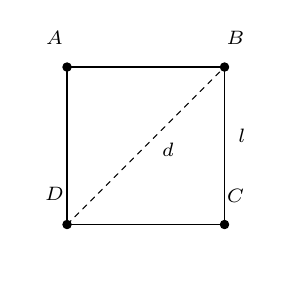
\begin{tikzpicture}[line cap=round,line join=round,>=triangle 45,x=1.0cm,y=1.0cm]
\clip(-1.5,-1.5) rectangle (1.5,1.5);
\draw (-1.,1.)-- (1.,1.);
\draw (1.,1.)-- (1.,-1.);
\draw (1.,-1.)-- (-1.,-1.);
\draw (-1.,-1.)-- (-1.,1.);
\draw [dash pattern=on 2pt off 2pt] (-1.,-1.)-- (1.,1.);
\begin{scriptsize}
\draw [fill=black] (-1.,1.) circle (1.5pt);
\draw[color=black] (-1.16,1.37) node {$A$};
\draw [fill=black] (1.,1.) circle (1.5pt);
\draw[color=black] (1.14,1.37) node {$B$};
\draw [fill=black] (1.,-1.) circle (1.5pt);
\draw[color=black] (1.14,-0.63) node {$C$};
\draw [fill=black] (-1.,-1.) circle (1.5pt);
\draw[color=black] (-1.16,-0.61) node {$D$};
\draw[color=black] (1.22,0.13) node {$l$};
\draw[color=black] (0.28,-0.05) node {$d$};
\end{scriptsize}
\end{tikzpicture}
\end{document}